\newpage
\chapter{Introduction}
Given the report from ACEA \cite{ACEA2021} we can see that the circulating fleets in EU have an average age of 13 years and with a predominance of Diesel powered as we can see in the Figure \ref{fig:hdpower}

%\cite{hdpower}

\begin{figure}[h]
\centering
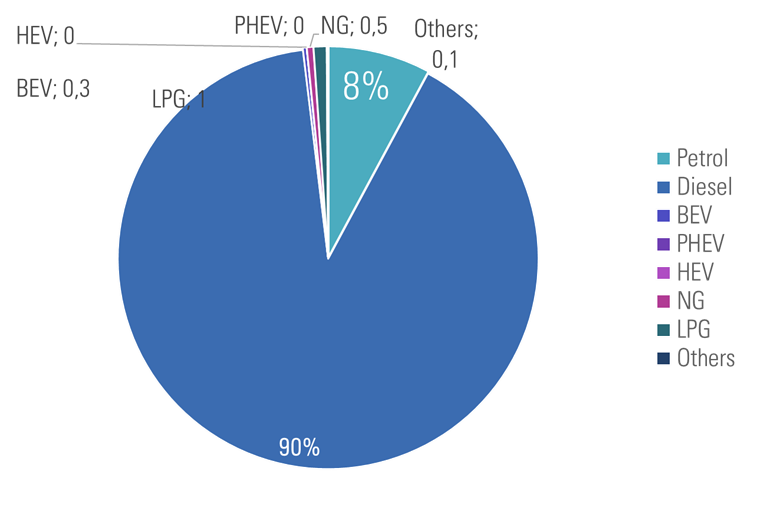
\includegraphics[width=0.8\textwidth]{Chapters/Pictures/grafico_diesel.png}
\caption{Powered Graph}
\label{fig:hdpower}
\end{figure}



So in compliance with the sustainability goals given by the UN it is necessary to renew also the Heavy duty compart. To do that we have 3 main options that we present in Table \ref{tab:dieselalternative}


\begin{table}[h]
\centering
\begin{tabular}{|l|l|l|}
\hline
\multicolumn{1}{|c|}{\textbf{Type of fuel}} & \multicolumn{1}{c|}{\textbf{PROS}}                                                                                                                              & \multicolumn{1}{c|}{\textbf{CONS}}                                                                                                \\ \hline
\textbf{Biofuels}                           & Derivable from waste products                                                                                                                                   & Still emit $CO_2$ during use                                                                                                      \\ \hline
\textbf{Electric}                           & \begin{tabular}[c]{@{}l@{}}$100\%$ clean during use\\ \\ Possible to couple the vehicle \\ \\ with a fixed infrastructure \\ \\ (OVH contact line)\end{tabular} & \begin{tabular}[c]{@{}l@{}}Cleanness depend on energetic mix\\ \\ Charging infrastructure\\ \\ Weight of the battery\end{tabular} \\ \hline
\textbf{FCEV}                               & \begin{tabular}[c]{@{}l@{}}$100\%$ clean during use\\ \\ Higher energy density\end{tabular}                                                                     & Lower volumetri density                                                                                                           \\ \hline
\end{tabular}
\caption{Pros and Cons of the possible alternative to diesel}
\label{tab:dieselalternative}
\end{table}


As said in a recent book the Electric batteries for Heay Duty are not so conviniebt so we will focus on the $H_2$ technologies.
\cite{Mazzo2021}

\newpage

\textit{In this section, provide a brief description of involved technologies, applications, state-of-the-art including actual size of systems, level of development, performances.}

\textit{Please, provide references/sources for the information in this section.}

\textit{3-6 pages (all the section)}

\section{Sate of the Art}